\documentclass[a4paper]{article}
\usepackage[english]{babel}
\usepackage[utf8]{vietnam}

%\usepackage{vntex}

%\usepackage[english,vietnam]{babel}
%\usepackage[utf8]{inputenc}

%\usepackage[utf8]{inputenc}
%\usepackage[francais]{babel}
\usepackage{a4wide,amssymb,epsfig,latexsym,multicol,array,hhline,fancyhdr}

\usepackage{amsmath}
\usepackage{lastpage}
\usepackage[lined,boxed,commentsnumbered]{algorithm2e}
\usepackage{enumerate}
\usepackage{color}
\usepackage{graphicx}                           
% Standard graphics package
\usepackage{listings}
\lstset{frame=tb,
  language=Python,
  aboveskip=3mm,
  belowskip=3mm,
  showstringspaces=false,
  columns=flexible,
  basicstyle={\small\ttfamily},
  numbers=none,
  numberstyle=\tiny\color{gray},
  keywordstyle=\color{blue},
  commentstyle=\color{dkgreen},
  stringstyle=\color{mauve},
  breaklines=true,
  breakatwhitespace=true,
  tabsize=3
}
\definecolor{dkgreen}{rgb}{0,0.6,0}
\definecolor{gray}{rgb}{0.5,0.5,0.5}
\definecolor{mauve}{rgb}{0.58,0,0.82}
\usepackage{array}
\usepackage{tabularx, caption}
\usepackage{multirow}
\usepackage{multicol}
\usepackage{rotating}
\usepackage{graphics}
\usepackage[a4paper,left=2cm,right=2cm,top=1.8cm,bottom=2.8cm]{geometry}
\usepackage{setspace}
\usepackage{epsfig}
\usepackage{tikz}
\usetikzlibrary{arrows,snakes,backgrounds}
\usepackage[unicode]{hyperref}
%can file puenc.def trong thu muc goc de option [unicode] tao ra bookmark bang tieng Viet
\hypersetup{urlcolor=blue,linkcolor=black,citecolor=black,colorlinks=true} 
%\usepackage{pstcol}                                
% PSTricks with the standard color package

\newtheorem{theorem}{{\bf Theorem}}
\newtheorem{property}{{\bf Property}}
\newtheorem{proposition}{{\bf Proposition}}
\newtheorem{corollary}[proposition]{{\bf Corollary}}
\newtheorem{lemma}[proposition]{{\bf Lemma}}


%\usepackage{fancyhdr}
\setlength{\headheight}{40pt}
\pagestyle{fancy}
\fancyhead{} % clear all header fields
\fancyhead[L]{
 \begin{tabular}{rl}
    \begin{picture}(25,15)(0,0)
    \put(0,-8){
\includegraphics[width=8mm, height=8mm]{hcmut.png}}
    %\put(0,-8){\epsfig{width=10mm,figure=hcmut.eps}}
   \end{picture}&
    %
\includegraphics[width=8mm, height=8mm]{hcmut.png} & %
    \begin{tabular}{l}
        \textbf{\bf \ttfamily Trường Đại học Bách Khoa - Đại học Quốc gia TP.HCM}\\
        \textbf{\bf \ttfamily Bộ môn Điều khiển \& Tự động}
    \end{tabular}   
 \end{tabular}
}
\fancyhead[R]{
    \begin{tabular}{l}
        \tiny \bf \\
        \tiny \bf 
    \end{tabular}  }
\fancyfoot{} % clear all footer fields
\fancyfoot[L]{\scriptsize \ttfamily Bài tập - Mạng Nơ-ron Tích chập \& Hồi tiếp, 04/2021}
\fancyfoot[R]{\scriptsize \ttfamily {\thepage}/\pageref{LastPage}}
\renewcommand{\headrulewidth}{0.3pt}
\renewcommand{\footrulewidth}{0.3pt}


%%%
\setcounter{secnumdepth}{4}
\setcounter{tocdepth}{3}
\makeatletter
\newcounter {subsubsubsection}[subsubsection]
\renewcommand\thesubsubsubsection{\thesubsubsection .\@alph\c@subsubsubsection}
\newcommand\subsubsubsection{\@startsection{subsubsubsection}{4}{\z@}%
                                     {-3.25ex\@plus -1ex \@minus -.2ex}%
                                     {1.5ex \@plus .2ex}%
                                     {\normalfont\normalsize\bfseries}}
\newcommand*\l@subsubsubsection{\@dottedtocline{3}{10.0em}{4.1em}}
\newcommand*{\subsubsubsectionmark}[1]{}
\makeatother


\begin{document}

\begin{titlepage}

\begin{center}
TRƯỜNG ĐẠI HỌC BÁCH KHOA - ĐẠI HỌC QUỐC GIA TP.HCM\\
BỘ MÔN ĐIỀU KHIỂN \& TỰ ĐỘNG
\end{center}

\vspace{1cm}

\begin{figure}[h!]
\begin{center}

\includegraphics[width=3cm]{hcmut.png}
\end{center}
\end{figure}

\vspace{1cm}


\begin{center}
\begin{tabular}{c}
\multicolumn{1}{l}{\textbf{{\Large TRÍ TUỆ NHÂN TẠO TRONG ĐIỀU KHIỂN}}}\\
~~\\
\hline
\\
\multicolumn{1}{l}{\textbf{{\Large Bài tập}}}\\
\\
\textbf{\Huge Mạng Nơ-ron Tích chập \& Hồi tiếp}\\
\\
\hline
\end{tabular}
\end{center}

\vspace{3cm}

\begin{table}[h]
\begin{tabular}{rrl}

\hspace{5 cm} & GVHD: Phạm Việt Cường & (pvcuong@hcmut.edu.vn)\\
& Lớp: L01, & Nhóm: 17\\
& Thành viên: & Nguyễn Thành Trung - 1814515 \\
& & Hoàng Đình Toản - 1814379\\
& & Đào Minh Triết - 1814426

\end{tabular}
\end{table}

\begin{center}
{\footnotesize Hồ Chí Minh, 04/2021}
\end{center}
\end{titlepage}


%\thispagestyle{empty}
\newpage
\tableofcontents
\newpage


%%%%%%%%%%%%%%%%%%%%%%%%%%%%%%%%%
\section{Đề bài}

\subsection{Bài 1} Ý nghĩa của \textbf{kết nối địa phương (\textit{local connectivity})} và \textbf{chia sẻ trọng số (\textit{shared weights})} trong mạng nơ-ron tích chập (\textit{Convolutional Neural Network} - CNN).
\subsection{Bài 2} Tính số thống số của mạng \href{https://en.wikipedia.org/wiki/AlexNet}{\textbf{AlexNet}}.
\subsection{Bài 3} Sử dụng tập dữ liệu có từ 100 ảnh có nhãn nằm trong 1000 nhãn của tập dữ liệu \href{http://www.image-net.org/download}{ImageNet}, thử nghiệm với ba mạng nơ-ron tích chập hiện đại bất kì, tính toán tỷ lệ lỗi top-1 và tỷ lệ lỗi top-5.
\subsection{Bài 4} Sử dụng phương thức học chuyển giao (\textit{transfer learning}) từ mạng AlexNet để phân loại một vài vật thể khác nhau trong một tập dữ liệu có khảong 100 ảnh.
\subsection{Bài 5} Thử nghiệm mô hình mạng nơ-ron hồi tiếp với 3 dữ liệu huấn luyện là:
\begin{table}[!h]
\centering
\begin{tabular}{|c|c|}
\hline
\textbf{dữ liệu} & \textbf{nhãn} \\ \hline
"h"              & "hello"       \\ \hline
"g"              & "green"       \\ \hline
"s"              & "start"       \\ \hline
\end{tabular}
\end{table}
\section{Về phần lập trình}
Chúng em sử dụng ngôn ngữ Python với sự hỗ trợ của thư viện PyTorch. Toàn bộ source code cũng như dữ liệu cho bài làm của chúng em có thể tìm thấy tại \href{https://github.com/dee-ex/hw\_cnn\_and\_rnn}{https://github.com/dee-ex/hw\_cnn\_and\_rnn}.
\newpage

%%%%%%%%%%%%%%%%%%%%%%%%%%%%%%%%%
\section{Lời giải}

\subsection{Bài 1}
Kết nối địa phương giúp cho mạng CNN có khả năng trích xuất những đặc trưng của một tấm ảnh đầu vào dựa vào một bộ lọc (\textit{filter/kernel}) tại nhiều vị trí khác nhau trên bức ảnh. Điều này giúp cho việc phát hiện những chi tiết trở nên tổng quát hơn vì ta chia nhỏ vùng ra để xem xét. Việc trích xuất đặc trưng này không chỉ diễn ra theo chiều rộng và cao mà còn theo chiều sâu của đầu vào.\\
Việc chia sẻ trọng số là để cho bộ lọc không chỉ có khả năng kết nối địa phương ở một vài ví trị nhất định mà phải là tất cả vị trí của dữ liệu đầu vào vì ta không biết trước rằng thứ ta muốn trích xuất nằm cụ thể ở một vị trí cho trước. Nếu muốn trích xuất nhiều đặc trưng, ta chỉ cần tăng số bộ lọc lên.

\subsection{Bài 2}
\begin{figure}[h!]
\centering
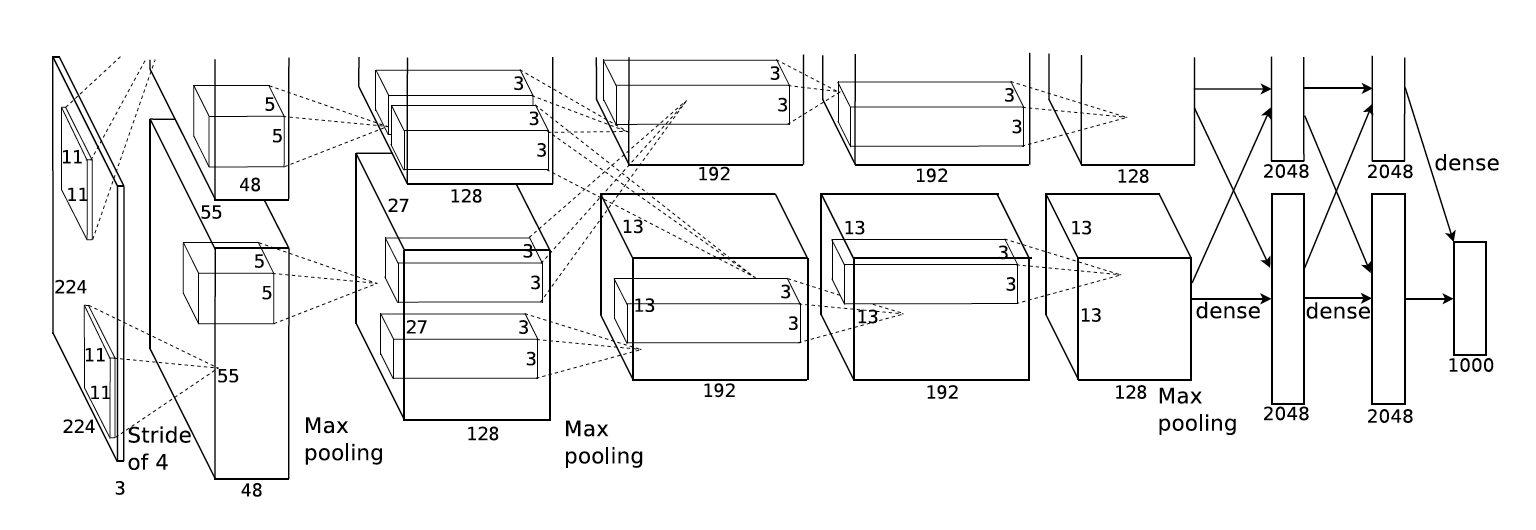
\includegraphics[width=17cm]{images/alexnet.png}
\caption*{Kiến trúc mạng AlexNet}
\end{figure}

\noindent
Từ đây, ta có thể tính toán số thông số (\textit{weights} $+$ \textit{biases}) của mỗi tầng như sau:

\begin{table}[!h]
\centering
{\renewcommand{\arraystretch}{1.8}
\begin{tabular}{|c|l|l|}
\hline
\textbf{Tầng} & \multicolumn{1}{c|}{\textbf{Số thông số}} & \multicolumn{1}{c|}{\textbf{Tổng số thông số}}\\ \hline
Conv-1 & $(11 \times 11 \times 3 + 1)\times 48 \times 2 = 34,944$ & $34,944$ \\\hline
Conv-2 & $(5 \times 5 \times 48 \times 2 + 1)\times 128 \times 2 = 614,656$ & $654,600$ \\ \hline
Conv-3 & $(3 \times 3 \times 128 \times 182 + 1)\times 192 \times 2 = 885,120$ & $1,539,720$ \\ \hline
Conv-4 & $(3 \times 3 \times 192 \times 2 + 1)\times 192 \times 2 = 1,327,488$ & $2,867,208$ \\ \hline
Conv-5 & $(3 \times 3 \times 192 \times 2 + 1)\times 128 \times 2 = 884,992$ & $3,752,200$ \\ \hline
FC-1 & $(6 \times 6 \times 256 + 1)\times 2048 \times 2 = 37,752,832$ & $41,505,032$ \\ \hline
FC-2 & $(2048 \times 2 + 1)\times 2048 \times 2 = 16,781,312$ & $58,286,344$ \\ \hline
FC-3 & $(2048 \times 2 + 1)\times 1000 = 4,097,000$ & $62,378,344$ \\ \hline
\end{tabular}} \quad
\end{table}

\subsection{Bài 3}\label{bai3}
Tập dữ liệu bao gồm 101 ảnh (định dạng \texttt{.jpg}) thuộc 101 lớp khác nhau được chúng em chọn ngẫu nhiên trong 1000 lớp của tập dữ liệu ImageNet.\\
Để thuận tiện cho việc lập trình, chúng em sử dụng nhãn của ảnh đề đặt tên cho ảnh. Tức là mỗi tấm ảnh trong tập dữ liệu sẽ có định dạng tên \texttt{label.jpg}.\\
Ba mạng nơ-ron được đưa ra thử nghiệm là: \textbf{AlexNet}, \textbf{GoogLeNet} và \textbf{ResNet}.

\subsubsection{Mạng AlexNet}
Đầu tiên, ta cần phải tải các thư viện cần thiết về.
\begin{lstlisting}
from torchvision import transforms
from torchvision import models
import torch

from PIL import Image
import os
\end{lstlisting}
Ta cần đọc được tên các ảnh, để từ đó trích xuất nhãn cũng như đọc ảnh cho việc thử nghiệm với mô hình.
\begin{lstlisting}
filenames = os.listdir("./images")

print(filenames[:3])
\end{lstlisting}
\begin{verbatim}
["volcano.jpg", "toaster.jpg", "forklift.jpg"]    
\end{verbatim}
Từ những tên file như vậy, ta có thể trích xuất label cũng như đọc ảnh.
\begin{lstlisting}
labels = [fname.split(".")[0] for fname in filenames]
imgs = [Image.open("./images/" + fname) for fname in filenames]
print(labels[:3], len(imgs))
\end{lstlisting}
\begin{verbatim}
["volcano", "toaster", "forklift"] 101
\end{verbatim}
Tiếp đến, ta sẽ tạo một transformer để biến đổi ảnh đầu vào của chúng ta phù hợp với đầu vào của mạng. Sau đó đưa từng ảnh qua transformer để tạo ra tensor tương ứng. Tất cả các tensor sẽ được lưu vào một tensor (N, channel, width, height).
\begin{lstlisting}
transformer = transforms.Compose([transforms.Resize(256),
                                  transforms.CenterCrop(224),
                                  transforms.ToTensor(),
                                  transforms.Normalize(
                                      mean=[.485, .456, .406],
                                      std=[.229, .224, .225]
                                  )]

transformed_imgs = torch.empty(0, 3, 224, 224)

for img in imgs:
  tf_img = transformer(img)
  tensor_tf_img = torch.unsqueeze(tf_img, 0)
  transformed_imgs = torch.cat((transformed_imgs, tensor_tf_img), dim=0)

print(transformed_imgs.shape)
\end{lstlisting}
\begin{verbatim}
torch.Size([101, 3, 224, 224])
\end{verbatim}
Vậy là bước tiền xử lí của chúng ta đã xong, bây giờ chúng sẽ đến bước tải mô hình về và thử nghiệm.
\begin{lstlisting}
alexnet = models.alexnet(pretrained=True)
print(alexnet)
\end{lstlisting}
\begin{verbatim}
AlexNet(
  (features): Sequential(
    (0): Conv2d(3, 64, kernel_size=(11, 11), stride=(4, 4), padding=(2, 2))
    (1): ReLU(inplace=True)
    (2): MaxPool2d(kernel_size=3, stride=2, padding=0, dilation=1, ceil_mode=False)
    (3): Conv2d(64, 192, kernel_size=(5, 5), stride=(1, 1), padding=(2, 2))
    (4): ReLU(inplace=True)
    (5): MaxPool2d(kernel_size=3, stride=2, padding=0, dilation=1, ceil_mode=False)
    (6): Conv2d(192, 384, kernel_size=(3, 3), stride=(1, 1), padding=(1, 1))
    (7): ReLU(inplace=True)
    (8): Conv2d(384, 256, kernel_size=(3, 3), stride=(1, 1), padding=(1, 1))
    (9): ReLU(inplace=True)
    (10): Conv2d(256, 256, kernel_size=(3, 3), stride=(1, 1), padding=(1, 1))
    (11): ReLU(inplace=True)
    (12): MaxPool2d(kernel_size=3, stride=2, padding=0, dilation=1, ceil_mode=False)
  )
  (avgpool): AdaptiveAvgPool2d(output_size=(6, 6))
  (classifier): Sequential(
    (0): Dropout(p=0.5, inplace=False)
    (1): Linear(in_features=9216, out_features=4096, bias=True)
    (2): ReLU(inplace=True)
    (3): Dropout(p=0.5, inplace=False)
    (4): Linear(in_features=4096, out_features=4096, bias=True)
    (5): ReLU(inplace=True)
    (6): Linear(in_features=4096, out_features=1000, bias=True)
  )
)}
\end{verbatim}
\begin{lstlisting}
alexnet.eval()

outputs = alexnet(transformed_imgs)
softout = torch.nn.functional.softmax(outputs, dim=-1)

print(softout.shape)
print(softout[:3, :5]
\end{lstlisting}
Kết quả dưới đây là 3 giá trị đầu ra của 3 đầu vào tương ứng. Mỗi đầu ra là 5 xác suất đầu tiên của tầng đầu ra.
\begin{verbatim}
torch.Size([101, 1000])
tensor([[1.1555e-11, 1.0505e-07, 1.5457e-11, 1.5857e-11, 2.4310e-12],
        [4.0361e-11, 1.0589e-09, 4.2571e-11, 7.8262e-12, 1.0931e-10],
        [1.5682e-12, 8.0843e-10, 8.0722e-13, 4.2640e-13, 5.1082e-13]],
       grad_fn=<SliceBackward>)
\end{verbatim}

\noindent
Để ý rằng, đầu ra mạng AlexNet của Pytorch không phải là một tầng softmax, do đó chúng ta cần thêm một bước tính softmax sau khi nhận được đầu ra.\\
Chúng ta cần tìm \texttt{argmax}, vậy nên ta có thể sắp xếp lại vector đầu ra theo giá trị giảm dần để dễ dàng xử lí.
\begin{lstlisting}
_, indices = torch.sort(softout, descending=True)

print(softout[0, indices[0, :5]]
\end{lstlisting}
Kiểm tra 5 xác suất cao nhất của đầu vào đầu tiên.
\begin{verbatim}
tensor([9.9999e-01, 9.7399e-07, 9.1711e-07, 4.3994e-07, 2.6995e-07],
       grad_fn=<IndexBackward>)
\end{verbatim}
Cuối cùng, ta sẽ lấy 1000 lớp của dữ liệu ImageNet để đối chiếu kiểm tra tỷ lệ lỗi top-1 và top-5.
\begin{lstlisting}
with open("imagenet_classes.txt") as f:
  classes = [line.strip() for line in f.readlines()]
  
count_top1 = 0
count_top5 = 0
N = indices.shape[0]

for i in range(N):
  if classes[indices[i, 0]].startswith(labels[i]):
    count_top1 += 1
    count_top5 += 1
  elif classes[indices[i, 1]].startswith(labels[i]):
    count_top5 += 1
  elif classes[indices[i, 2]].startswith(labels[i]):
    count_top5 += 1
  elif classes[indices[i, 3]].startswith(labels[i]):
    count_top5 += 1
  elif classes[indices[i, 4]].startswith(labels[i]):
    count_top5 += 1

print("top-1 error rate", 100 * (1 - count_top1/N))
print("top-5 error rate", 100 * (1 - count_top5/N))
\end{lstlisting}
\begin{verbatim}
top-1 error rate 19.8019801980198
top-5 error rate 8.910891089108908
\end{verbatim}

\noindent
Với 101 tấm ảnh thử nghiệm, tỷ lệ lỗi top-1 là $19.8\%$, thấp hơn so với kết quả của bài báo gốc $17.7\%$. Còn tỷ lệ lỗi top-5 là $8.9\%$, cũng thấp hơn so với kết quả của bài báo gốc $8.1\%$.\\
Tỷ lệ lỗi ở top-1 cũng cao hơn tỷ lệ lỗi ở top-5, cụ thể là hơn $10.9\%$, điều này là hiển nhiên vì ở trong top-1 thì chắc chắn ở trong top-5, nhưng ngược lại thì chưa chắc.\\
Kiểm tra một vài bức ảnh, ta thấy mô hình của ta nhận diện giống như bộ não của chúng ta hoạt động khi sự nhầm lần là nhầm lẫn giữa những thứ tương tự.
\begin{figure}[h!]
\centering
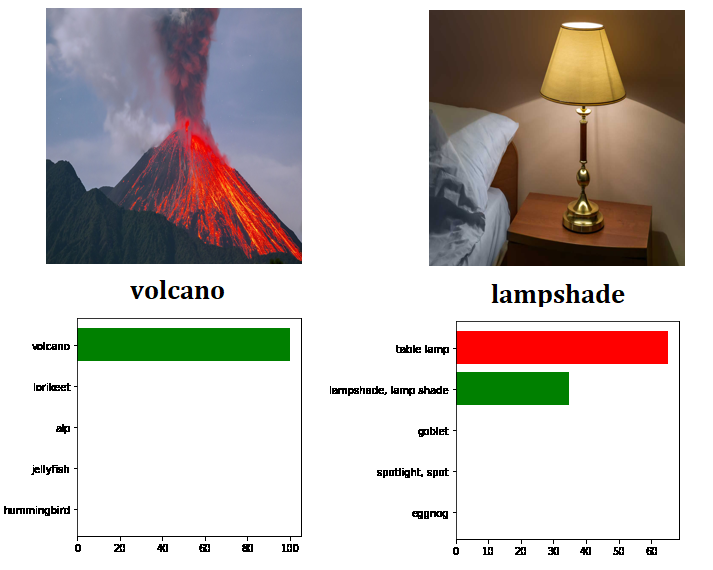
\includegraphics[width=15cm]{images/res1.PNG}
\caption*{Những ảnh được mô hình phân loại chính xác cao}
\end{figure}

\noindent
Ở tấm hình cái dĩa, hoa văn của nó đã làm cho mô hình dự đoán sai ra những nhãn khác, điều này khá khó tránh khỏi khi những đặc trưng này nổi bật hơn cả so với những đặc trưng khác của cái dĩa.
\newpage

\begin{figure}[h!]
\centering
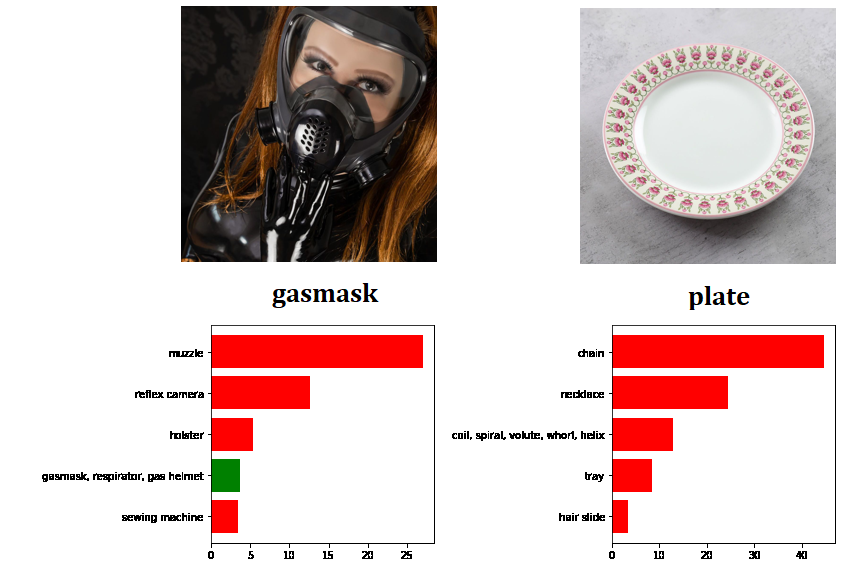
\includegraphics[width=15cm]{images/res2.PNG}
\caption*{Những ảnh được mô hình phân loại chưa chính xác cao}
\end{figure}

\noindent
Dẫu vậy, ta vẫn thấy tỷ lệ lỗi vẫn khá cao và vẫn còn bị nhiễu bởi các chi tiết xung quanh vì mô hình này ra đời đã lâu. Ta mong sẽ có kết quả tốt hơn khi thử nghiệm với các mô hình mới hơn.
\subsubsection{Mạng GoogLeNet và ResNet}
Quá trình cũng không khác gì so với mạng AlexNet.
\begin{lstlisting}
googlenet = models.googlenet(pretrained=True)
googlenet.eval()

outputs = googlenet(transformed_imgs)
softout = torch.nn.functional.softmax(outputs, dim=-1)

with open("imagenet_classes.txt") as f:
  classes = [line.strip() for line in f.readlines()]

top5_softmax, top5_idx = torch.topk(softout, 5, dim=-1)

count_top1 = 0
count_top5 = 0
N = top5_idx.shape[0]

for i in range(N):
  for j in range(5):
    if classes[top5_idx[i, j]].startswith(labels[i]):
      count_top5 += 1
      break

  count_top1 += 1 if classes[top5_idx[i, 0]].startswith(labels[i]) else 0

print("top-1 error rate", 100 * (1 - count_top1/N))
print("top-5 error rate", 100 * (1 - count_top5/N))
\end{lstlisting}
\begin{verbatim}
top-1 error rate 10.89108910891089
top-5 error rate 4.950495049504955
\end{verbatim}
Còn đây là kết quả của mạng ResNet:
\begin{lstlisting}
resnet = models.resnet18(pretrained=True)
...
print("top-1 error rate", 100 * (1 - count_top1/N))
print("top-5 error rate", 100 * (1 - count_top5/N))
\end{lstlisting}
\begin{verbatim}
top-1 error rate 11.881188118811881
top-5 error rate 6.930693069306926
\end{verbatim}
Từ đó, ta có bảng so sánh tỷ lệ lỗi top-1 và top-5 của 3 mô hình trên như sau:
\begin{table}[!h]
\centering
{\renewcommand{\arraystretch}{1}
\begin{tabular}{|l|c|c|}
\hline
\textbf{Mô hình} & \textbf{Top-1} & \textbf{Top-5} \\ \hline
AlexNet          & $19.80\%$              & $8.91\%$              \\ \hline
GoogLeNet        & $\mathbf{10.89\%}$              & $\mathbf{4.95\%}$              \\ \hline
ResNet           & $11.88\%$              & $6.93\%$              \\ \hline
\end{tabular}}
\end{table}

\noindent
Dễ thấy rằng, cả 2 mô hình trên đều có sự cải thiện so với mô hình mạng AlexNet. Tỷ lệ lỗi top-1 đã giảm từ $19.8\%$ xuống $10.89\%$ (giảm $19.8/10.89 \approx 1.81$ lần) đối với mạng GoogLeNet và $11.88\%$ (giảm $19.8/11.88 \approx 1.67$ lần) đối với mạng ResNet. Tỷ lệ lỗi top-5 đã giảm từ $8.91\%$ xuống $4.95\%$ (giảm $8.91/4.95 \approx 1.8$ lần) đối với mạng GoogLeNet và $6.93\%$ (giảm $8.91/6.93 \approx 1.29$ lần) đối với mạng ResNet.\\
Một điều nữa mà GoogLeNet và ResNet cải thiện được nữa là kích thước cũng như là thông số mô hình nhỏ hơn đáng kể cho với AlexNet. Chi tiết tham khảo \href{https://www.mathworks.com/help/deeplearning/ug/pretrained-convolutional-neural-networks.html}{MathWorks - Pretrained Deep Neural Networks}.\\
Để thấy rõ sự cải thiện của mạng GoogLeNet so với Alexnet, ta sẽ kiểm tra lại 2 hình ở mạng AlexNet có sai số khá lớn.
\begin{figure}[h!]
\centering
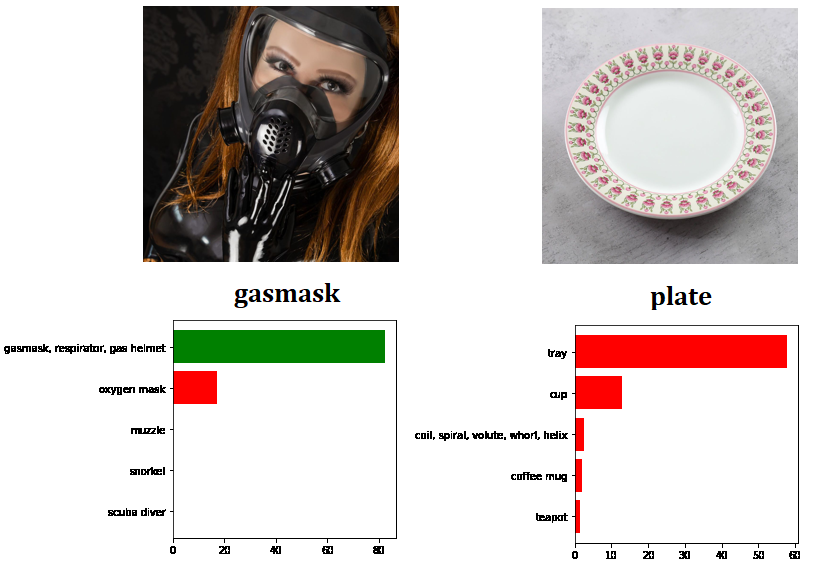
\includegraphics[width=15cm]{images/res3.PNG}
\caption*{Ảnh được phân loại chưa chính xác cao bằng AlexNet được phân loại lại bởi GoogLeNet}
\end{figure}

\noindent
Nhìn chung, kết quả có khả quan hơn, khi giờ đây ở ảnh có nhãn là \texttt{gasmask} đã lên top-1. Với ảnh có nhãn là \texttt{plate}, tuy chưa lên được top-5, tuy nhiên mô hình cũng đã loại bỏ được nhiễu ở hoa văn xung quanh và tìm được những vật có tính chất tương tự với cái dĩa.

\subsection{Bài 4}
Tập dữ liệu về các linh kiện điện tử đơn giản gồm 128 ảnh (định dạng \texttt{.jpg}) thuộc 10 lớp khác nhau (chi tiết trong thư mục \texttt{datasets}). Trong đó số train-validation-test là 80-24-24. Đây là những dữ liệu được chúng em tự tay thu thập. Trong quá trình thực hiện quá trình, có một vài sai xót trong việc xử lí camera nên một vài hình ảnh bị mờ, nhoè, không rõ nét. Tuy vậy, chúng em nhận thấy đây cũng có thể là một thử tách cho mô hình để đánh giá xem mô hình có đủ tốt để vượt qua hay không.\\
Không giống như \hyperref[bai3]{\textbf{Bài 3}}, ở bài này, ta sẽ thay đổi một vài chi tiết của mô hình ở những tầng cuối cùng để có thể phù hợp với bài toán của chúng ta hơn. Cụ thể là phân loại những thiết bị linh kiện điện tử gần gũi với những sinh viên khoa điện, nhưng lại không có trong tập dữ liệu ImageNet. Vậy nên ta cũng cần phải huấn luyện lại mô hình. Đầu tiên, ta sẽ tạo những thứ cơ bản cho việc tải dữ liệu để huấn luyện và xác thực.
\begin{lstlisting}
import torch
import torch.nn as nn
from torch.utils.data import DataLoader
from torchvision import datasets, models, transforms

import numpy as np
import matplotlib.pyplot as plt

import time

from PIL import Image

transformer = transforms.Compose([transforms.Resize(256),
                                  transforms.CenterCrop(224),
                                  transforms.ToTensor(),
                                  transforms.Normalize(
                                      mean=[0.485, 0.456, 0.406],
                                      std=[0.229, 0.224, 0.225]),
                                  ])

batch_size = 8
num_classes = 10
data = {
  "train": datasets.ImageFolder("./datasets/train", transformer),
  "valid": datasets.ImageFolder("./datasets/validation", transformer)
}
idx_to_class = {v: k for k, v in data["train"].class_to_idx.items()}

train_size, valid_size = len(data["train"]), len(data["valid"])

train_loader = DataLoader(data["train"], batch_size, True)
valid_loader = DataLoader(data["valid"], batch_size, True)
\end{lstlisting}
Tiếp theo, ta sẽ lấy mô hình mạng AlexNet đã được huấn luyện rồi và chỉnh sửa lại một chút ở tầng cuối cùng. Như ở \hyperref[bai3]{\textbf{Bài 3}} ta đã thấy, tầng đầu ra là tầng \textbf{6}, nên ta sẽ thay đổi ở tầng này.
\begin{lstlisting}
alexnet = models.alexnet(pretrained=True)
alexnet.classifier[6] = nn.Linear(4096, num_classes)
alexnet.classifier.add_module("7", nn.LogSoftmax(dim = 1))

loss_func = nn.NLLLoss()
optimizer = torch.optim.Adam(alexnet.parameters())
\end{lstlisting}
Ở tầng đầu ra của mô hình chúng ta, việc thêm một tầng \texttt{LogSoftmax} sẽ có kết quả tốt hơn khi huấn luyện khi kết hợp với \texttt{NLLLoss}.\footnote{Data Science, \lq What is the advantage of using log softmax instead of softmax\rq, \href{https://bit.ly/3sIU4wV}{https://bit.ly/3sIU4wV}}
\begin{lstlisting}
def train_and_validate(model, loss_criterion, optimizer, epochs=25):
  start = time.time()
  history = []
  best_acc = .0

  for epoch in range(epochs):
    epoch_start = time.time()
    model.train()

    train_loss, train_acc = .0, .0
    valid_loss, valid_acc = .0, .0
    
    for i, (inputs, labels) in enumerate(train_data_loader):
      inputs = inputs
      labels = labels
      
      optimizer.zero_grad()
      
      outputs = model(inputs)
      
      loss = loss_criterion(outputs, labels)
      
      loss.backward()
      
      optimizer.step()
      
      train_loss += loss.item() * inputs.size(0)
      
      ret, predictions = torch.max(outputs.data, 1)
      correct_counts = predictions.eq(labels.data.view_as(predictions))
      
      acc = torch.mean(correct_counts.type(torch.FloatTensor))
      
      train_acc += acc.item() * inputs.size(0)
        
    with torch.no_grad():
      model.eval()

      for j, (inputs, labels) in enumerate(valid_data_loader):
        inputs = inputs
        labels = labels

        outputs = model(inputs)

        loss = loss_criterion(outputs, labels)

        valid_loss += loss.item() * inputs.size(0)

        ret, predictions = torch.max(outputs.data, 1)
        correct_counts = predictions.eq(labels.data.view_as(predictions))

        acc = torch.mean(correct_counts.type(torch.FloatTensor))

        valid_acc += acc.item() * inputs.size(0)

        
    avg_train_loss = train_loss/train_data_size 
    avg_train_acc = train_acc/train_data_size

    avg_valid_loss = valid_loss/valid_data_size 
    avg_valid_acc = valid_acc/valid_data_size

    history.append([avg_train_loss, avg_valid_loss, avg_train_acc, avg_valid_acc])
            
    epoch_end = time.time()

    print("Epoch : {}, trn_loss: {:.4f}, trn_acc: {:.4f}%, val_loss : {:.4f}, val_acc: {:.4f}%, Time: {:.4f}s".format(epoch+1, avg_train_loss, avg_train_acc*100, avg_valid_loss, avg_valid_acc*100, epoch_end-epoch_start))
      
  return model, history
\end{lstlisting}
Trong trường hợp muốn lưu giữ lại mô hình có kết quả tốt nhất, ta cũng có thể lưu lại mô hình qua mỗi epoch:
\begin{lstlisting}
torch.save(model, "model_" + str(epoch) + ".pt")
\end{lstlisting}
Mọi bước chuẩn bị đã xong, chọn số epoch và bước vào quá trình huấn luyện.
\begin{lstlisting}
num_epochs = 30
trained_model, history = train_and_validate(alexnet, loss_func, optimizer, num_epochs)
\end{lstlisting}
\begin{verbatim}
Epoch : 1, trn_loss: 2.5871, trn_acc: 16.2500%, val_loss : 1.9774, val_acc: 33.3333%, Time: 16.9606s
Epoch : 2, trn_loss: 2.2365, trn_acc: 17.5000%, val_loss : 2.2949, val_acc: 12.5000%, Time: 16.4911s
Epoch : 3, trn_loss: 2.3083, trn_acc: 8.7500%, val_loss : 2.2891, val_acc: 25.0000%, Time: 16.6145s
...
Epoch : 28, trn_loss: 2.2534, trn_acc: 16.2500%, val_loss : 2.2473, val_acc: 25.0000%, Time: 16.2459s
Epoch : 29, trn_loss: 2.2584, trn_acc: 16.2500%, val_loss : 2.2427, val_acc: 25.0000%, Time: 16.1560s
Epoch : 30, trn_loss: 2.2585, trn_acc: 16.2500%, val_loss : 2.2462, val_acc: 25.0000%, Time: 16.2874s
\end{verbatim}
\begin{figure}[h!]
\centering
{{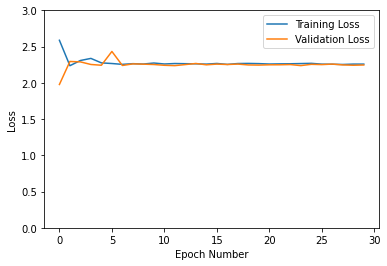
\includegraphics[width=8cm]{images/loss.png} }}
\qquad
{{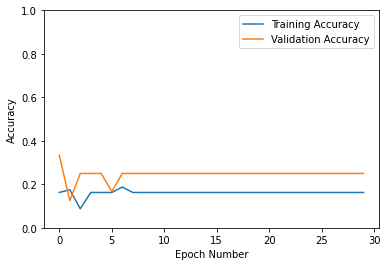
\includegraphics[width=8cm]{images/acc.png} }}
\caption*{Loss và Accuracy của hai quá trình training và validation}
\end{figure}
Kết quả có vẻ không như ta mong muốn, khi loss cao và không có dấu hiệu giảm, accuracy thì lại quá thấp ($< 50\%$) và cũng không có dấu hiệu tăng. Có lẽ ta không cần phải đem mô hình này đi thử nghiệm vì không lí nào mô hình lại có thể có thể dự đoán tốt với kết quả như thế này.\\
Sẽ ra sao nếu ta giữ lại những tầng trước đó của mô hình, và chỉ huấn luyện tầng mà ta thay đổi để tránh "làm hỏng" những tầng tích chập? Muốn giữ lại các thông số của mô hình cũ, ta cần phải \textbf{freeze} tất các lớp, sau đó thay thế những lớp ta muốn huấn luyện bằng một lớp mới. Cụ thể, nếu ta muốn giữ lại tất cả các lớp trước trừ lớp cuối cùng, thì bước khởi tạo mô hình trước khi huấn luyện cần phải làm như sau:
\begin{lstlisting}
alexnet = models.alexnet(pretrained=True)

for param in alexnet.parameters():
  param.requires_grad = False
\end{lstlisting}
Và khi ta thực hiện lại bước huấn luyện, may mắn thay, ta được kết quả hàm mất mát giảm như mong đợi.
\begin{verbatim}
Epoch : 1, trn_loss: 1.9950, trn_acc: 33.7500%, val_loss : 1.0423, val_acc: 70.8333%, Time: 6.4752s
Epoch : 2, trn_loss: 0.5381, trn_acc: 85.0000%, val_loss : 0.5710, val_acc: 91.6667%, Time: 6.3596s
Epoch : 3, trn_loss: 0.2200, trn_acc: 96.2500%, val_loss : 0.4143, val_acc: 95.8333%, Time: 6.4472s
Epoch : 4, trn_loss: 0.1230, trn_acc: 98.7500%, val_loss : 0.3881, val_acc: 95.8333%, Time: 6.4681s
...
Epoch : 27, trn_loss: 0.0079, trn_acc: 100.0000%, val_loss : 0.3143, val_acc: 95.8333%, Time: 6.2976s
Epoch : 28, trn_loss: 0.0096, trn_acc: 100.0000%, val_loss : 0.3323, val_acc: 95.8333%, Time: 6.3094s
Epoch : 29, trn_loss: 0.0119, trn_acc: 100.0000%, val_loss : 0.3013, val_acc: 95.8333%, Time: 6.3837s
Epoch : 30, trn_loss: 0.0084, trn_acc: 100.0000%, val_loss : 0.2886, val_acc: 95.8333%, Time: 6.4277s
\end{verbatim}

\begin{figure}[h!]
\centering
{{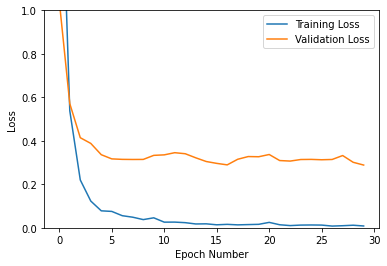
\includegraphics[width=8cm]{images/loss1.png} }}
\qquad
{{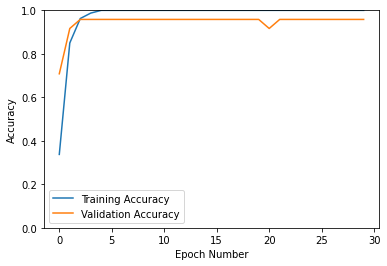
\includegraphics[width=8cm]{images/acc1.png} }}
\caption*{Loss và Accuracy của hai quá trình training và validation sau khi \textbf{freeze} các tầng phía trước}
\end{figure}

\noindent
Kết quả đã khả quan hơn, hãy xem thử tỷ lệ lỗi top-1 và top-3. Ở đây, ta sử dụng tỷ lệ lỗi top-3 thay vì top-5 vì số lượng lớp ít, việc sử dụng top-5 thì nó là một nửa số lớp, việc đánh giá sẽ thiên vị cho mô hình của chúng ta.
\begin{lstlisting}
import os

filenames = os.listdir("./datasets/test/")
imgs = [Image.open("./datasets/test/" + fname) for fname in filenames]

transformed_imgs = torch.empty(0, 3, 224, 224)

for img in imgs:
  tf_img = transformer(img)
  tensor_tf_img = torch.unsqueeze(tf_img, 0)
  transformed_imgs = torch.cat((transformed_imgs, tensor_tf_img), dim=0)

outputs = trained_model(transformed_imgs)
softout = nn.functional.softmax(outputs, dim=-1)
top3_softmax, top3_idx = torch.topk(softout, 3, dim=-1)

count_top1 = 0
count_top3 = 0
N = top3_idx.shape[0]

for i in range(N):
  for j in range(3):
    if filenames[i].startswith(idx_to_class[top3_idx[i, j].item()]):
      count_top3 += 1
      break

  count_top1 += 1 if filenames[i].startswith(idx_to_class[top3_idx[i, 0].item()]) else 0

print("top-1 error rate", 100 * (1 - count_top1/N))
print("top-3 error rate", 100 * (1 - count_top3/N))
\end{lstlisting}
\begin{verbatim}
top-1 error rate 20.833333333333336
top-3 error rate 8.333333333333337
\end{verbatim}
Không quá tệ, đặc biệt là khi các linh kiện mà ta phân loại cũng có sự tương đồng khá lớn giữa các linh kiện. Ta sẽ thấy rõ hơn điều này bằng cách xem chi tiết một vài kết quả.
\newpage
\begin{figure}[h!]
\centering
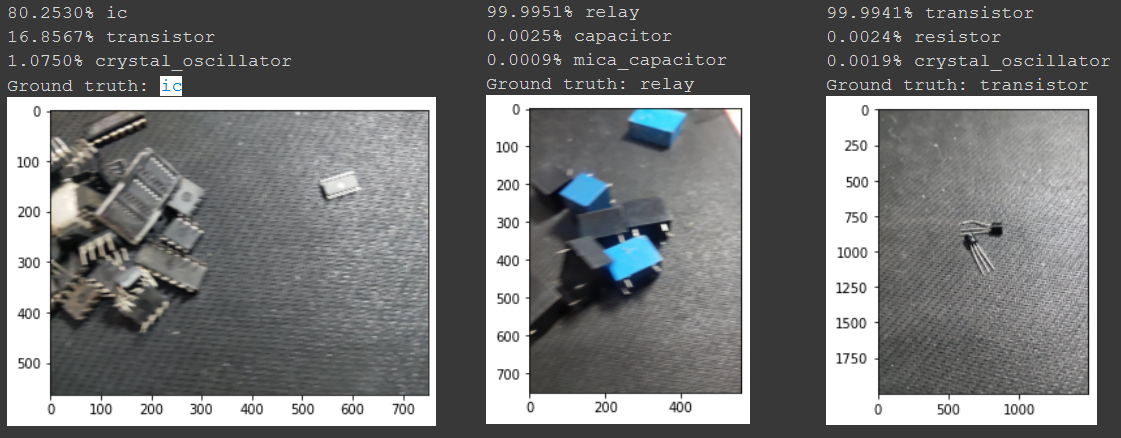
\includegraphics[width=15cm]{images/result1.PNG}
\caption*{Những linh kiện được mô hình phân loại chính xác cao}
\end{figure}

\noindent
Dễ thấy rằng, những hình này có hình khối và đặc điểm dễ dàng nhận dạng. Ví dụ như \textbf{ic} thì nhiều chân, \textbf{relay} thì khối như \textbf{ic}, nhưng lại ít chân hơn, còn \textbf{transistor} thì cũng ít chân như \textbf{relay} nhưng lại có kích thước nhỏ.
\begin{figure}[h!]
\centering
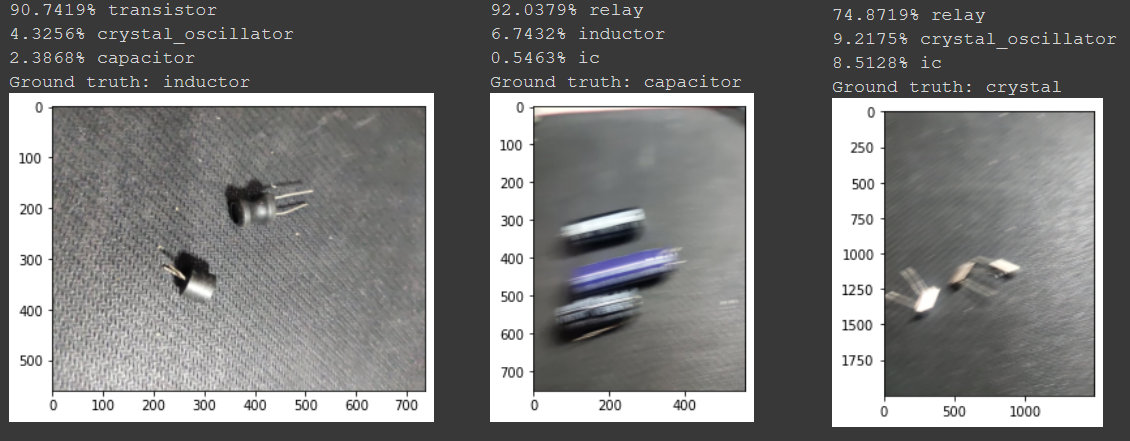
\includegraphics[width=15cm]{images/result2.PNG}
\caption*{Những linh kiện được mô hình phân loại chưa chính xác cao}
\end{figure}

\noindent
Hình ảnh \textbf{inductor} này thực sự khó với mô hình, vì dạng này chưa được huấn luyện cho mô hình, nên nhầm lẫn là điều hết sức bình thường, càng dễ hiểu hơn khi mô hình dữ đoán với những thứ khá tương đồng với \textbf{inductor} dạng như thế này là \textbf{transistor} hay là \textbf{thạch anh}.\\
Với hình ảnh \textbf{capacitor} không thể lọt vào top-3, ta thấy rằng ảnh này bị chụp thiếu chính xác, gây ra nhiễu lớn, cũng như bản thân con tụ cũng có chân ngắn, khó phân biệt so với những con tụ bình thường được chụp một cách rõ nét.\\
Về phần \textbf{thạch anh}, kết quả dự đoán khá bất ngờ khi top-3 lại có \textbf{relay} và \textbf{ic} vì cơ bản \textbf{thạch anh} và hai linh kiện kia không có mấy điểm chung. Nếu kết quả là \textbf{transistor} hoặc \textbf{mica capacitor} hay là \textbf{resistor} có lẽ sẻ dễ hiểu hơn.\\

\noindent
Nhìn chung, mô hình được huấn luyện có khả năng phân loại một số linh kiện điện tử đơn giản với độ chính xác khá cao, khoảng $\approx 80\%$ trong điều kiện hình ảnh rõ nét. Vẫn còn khá hạn chế với những ảnh bị nhiễu. Dẫu vậy, nếu được huấn luyện với tập dữ liệu tốt hơn, việc tăng độ chính xác là điều hoàn toàn khả thi.
\newpage
\subsection{Bài 5}
Vì mạng nơ-ron hồi tiếp chỉ mới tiếp cận, nên việc triển khai mô hình này chúng em xin phép không đi sâu vào phần giải thích thuật toán.\\
Nhưng trước tiên, để làm khoa học dữ liệu, ta cần phải có dữ liệu. Bước tiền xử lí dữ liệu, bước này không có gì đặc biệt về thuật toán, chỉ đơn giản là chuyển các dữ liệu đầu vào thành các one-hot vector.
\begin{lstlisting}
import torch
from torch import nn

words = ["hello", "green", "start"]

chars = set("".join(words))

int2char = dict(enumerate(chars))
char2int = {chr: idx for idx, chr in int2char.items()}

print(int2char)
print(char2int)
\end{lstlisting}
\begin{verbatim}
{0: "g", 1: "t", 2: "a", 3: "l", 4: "n", 5: "h", 6: "o", 7: "r", 8: "e", 9: "s"}
{"g": 0, "t": 1, "a": 2, "l": 3, "n": 4, "h": 5, "o": 6, "r": 7, "e": 8, "s": 9}
\end{verbatim}
Những công cụ \texttt{int2char} và \texttt{char2int} sẽ được sử dụng trong việc chuyển đổi sang one-hot vector cũng như là cho việc kiểm tra (\textit{test}).\\
Ta cần cắt bớt một kí tự cuối cho đầu vào, một kí từ đầu cho đầu ra. Sau đó chuyển đổi các dữ liệu kí tự sang dữ liệu số vì hiển nhiên các mô hình toán chỉ hiểu các con số. Và rồi cuối cùng chuyển đổi sang one-hot vector. Ta sẽ viết riêng một hàm để làm việc này, để tái sử dụng cho quá trình kiểm tra.
\begin{lstlisting}
inp, tar = [], []

for word in words:
  inp.append(word[:-1])
  tar.append(word[1:])

for i in range(len(words)):
  inp[i] = [char2int[chr] for chr in inp[i]]
  tar[i] = [char2int[chr] for chr in tar[i]]

print(inp)
print(tar

dict_size = len(char2int)
seq_len =  len(inp[0])
batch_size = len(words)

def one_hot_encode(seq, dict_size, seq_len, batch_size):
  features = torch.zeros((batch_size, seq_len, dict_size))

  for i in range(batch_size):
    for j in range(seq_len):
      features[i, j, seq[i][j]] = 1

  return features
  
inp_1hot = one_hot_encode(inp, dict_size, seq_len, batch_size)
print(inp_1hot.shape)
print(inp_1hot)
\end{lstlisting}
\begin{verbatim}
[[5, 8, 3, 3], [0, 7, 8, 8], [9, 1, 2, 7]]
[[8, 3, 3, 6], [7, 8, 8, 4], [1, 2, 7, 1]]
torch.Size([3, 4, 10])
tensor([[[0., 0., 0., 0., 0., 1., 0., 0., 0., 0.],
         [0., 0., 0., 0., 0., 0., 0., 0., 1., 0.],
         [0., 0., 0., 1., 0., 0., 0., 0., 0., 0.],
         [0., 0., 0., 1., 0., 0., 0., 0., 0., 0.]],

        [[1., 0., 0., 0., 0., 0., 0., 0., 0., 0.],
         [0., 0., 0., 0., 0., 0., 0., 1., 0., 0.],
         [0., 0., 0., 0., 0., 0., 0., 0., 1., 0.],
         [0., 0., 0., 0., 0., 0., 0., 0., 1., 0.]],

        [[0., 0., 0., 0., 0., 0., 0., 0., 0., 1.],
         [0., 1., 0., 0., 0., 0., 0., 0., 0., 0.],
         [0., 0., 1., 0., 0., 0., 0., 0., 0., 0.],
         [0., 0., 0., 0., 0., 0., 0., 1., 0., 0.]]])
\end{verbatim}
Sau khi có được dữ liệu, ta sẽ tiến hành xây dựng mô hình.
\begin{lstlisting}
class RNN(nn.Module):
  def __init__(self, inp_size, out_size, hidden_dim, n_layers):
    super(RNN, self).__init__()

    self.hidden_dim = hidden_dim
    self.n_layers = n_layers

    self.rnn = nn.RNN(inp_size, hidden_dim, n_layers, batch_first=True)

    self.fc = nn.Linear(hidden_dim, out_size)

  def forward(self, x):
    batch_size = x.shape[0]

    hidden = self.init_hidden(batch_size)

    out, hidden = self.rnn(x, hidden)

    out = out.contiguous().view(-1, self.hidden_dim)
    out = self.fc(out)

    return out, hidden

  def init_hidden(self, batch_size):
    hidden = torch.zeros(self.n_layers, batch_size, self.hidden_dim)

    return hidden
    
rnn = RNN(dict_size, dict_size, 12, 1)
\end{lstlisting}
Rồi đem mô hình đi huấn luyện bằng đại lương \textbf{cross entropy} và thuật toán tối ưu \textbf{Adam}. Vì lượng dữ liệu ít, nên việc huấn luyện cũng diễn ra nhanh chóng.
\begin{lstlisting}
target = torch.Tensor(tar)

n_epochs = 100
lr = .01

criterion = nn.CrossEntropyLoss()
optimizer = torch.optim.Adam(rnn.parameters(), lr)

for epoch in range(1, n_epochs + 1):
  optimizer.zero_grad()

  out, hidden = rnn(inp_1hot)
  loss = criterion(out, target.view(-1).long())
  loss.backward()
  optimizer.step()

  if not epoch % 10:
    print("Epoch:", epoch, "..... Loss:", loss.item())
\end{lstlisting}
\begin{verbatim}
Epoch: 10 ..... Loss: 1.7420676946640015
Epoch: 20 ..... Loss: 1.2189706563949585
Epoch: 30 ..... Loss: 0.7296259999275208
Epoch: 40 ..... Loss: 0.37214040756225586
Epoch: 50 ..... Loss: 0.18362826108932495
Epoch: 60 ..... Loss: 0.10042735189199448
Epoch: 70 ..... Loss: 0.06265192478895187
Epoch: 80 ..... Loss: 0.04381946101784706
Epoch: 90 ..... Loss: 0.03324601799249649
Epoch: 100 ..... Loss: 0.026623765006661415
\end{verbatim}
Ta sẽ đi xem kết quả của mô hình sau khi huấn luyện, nhưng trước tiên ta cần một số càm cần thiết để giúp quá trình này dễ dàng hơn.
\begin{lstlisting}
def predict(model, word):
  chars = [[char2int[chr] for chr in word]]
  onehot = one_hot_encoder(chars, dict_size, len(chars[0]), 1)

  out, hidden = model(onehot)

  prob = nn.functional.softmax(out[-1], dim=0).data

  char_idx = torch.max(prob, dim=0)[1].item()

  return int2char[char_idx], hidden
  
def sample(model, out_len, start):
  model.eval()

  start = start.lower()
  chars = [chr for chr in start]
  size = out_len - len(chars)

  for _ in range(size):
    chr, h = predict(model, chars)
    chars.append(chr)

  return "".join(chars)
\end{lstlisting}
Cuối cùng ta cũng đã tới được bước thú vị nhất, là xem kết quả dữ đoán của mô hình.
\begin{lstlisting}
test = ["h", "g", "s", "e", "t"]

for s in test:
  print(s, " -> ", sample(rnn, seq_len + 1, s))
\end{lstlisting}
\begin{verbatim}
h  ->  hello
g  ->  green
s  ->  start
e  ->  eello
t  ->  tarta
\end{verbatim}
Ta thấy rằng, với những lần thử nghiệm có dữ liệu đầu vào đã được đưa cho mô hình học thì kết quả nhận được hoàn toàn khớp với những gì chúng ta mong đợi. Tuy nhiên với những dữ liệu đầu vào mà mô hình chưa được học thì kết quả trả ra khá vô nghĩa. Điều này là dễ hiểu vì sự thiếu hụt dữ liệu cho việc huấn luyện mô hình trên, dẫn đến việc mô hình quá khớp, chỉ đang ghi nhớ chứ không thực sự là học.

%%%%%%%%%%%%%%%%%%%%%%%%%%%%%%%%%
\begin{thebibliography}{80}

    \bibitem{elistevens} Eli Stevens, Luca Antiga, Thomas Viehmann and Foreword by Soumith Chintala, Deep Learning with PyTorch, Manning Publications, New York (2020).

    \bibitem{floyhub} FloyHub, A Beginner’s Guide on Recurrent Neural Networks with PyTorch, \href{https://bit.ly/3n5RpvV}{https://bit.ly/3n5RpvV} (2019).
    
    \bibitem{learnopencv} Learn OpenCV, Understanding AlexNet, \href{https://bit.ly/2P5ZxA1}{https://bit.ly/2P5ZxA1} (2018).

    \bibitem{pytorch} PyTorch, AlexNet, \href{https://bit.ly/3sCwDF6}{https://bit.ly/3sCwDF6} (2017).
    
    \bibitem{pytorch} PyTorch, Finetuning Torchvision Models, \href{https://bit.ly/3grJCY6}{https://bit.ly/3grJCY6} (2017).
    
    \bibitem{pytorch} PyTorch, GoogLeNet, \href{https://bit.ly/3tBXym7}{https://bit.ly/3tBXym7} (2017).
    
    \bibitem{pytorch} PyTorch, torchvision.models, \href{https://bit.ly/3v3aFgg}{https://bit.ly/3v3aFgg} (2017).
    
    \bibitem{pytorch} PyTorch, Transfer Learning for Computer Vision Tutorial, \href{https://bit.ly/32tHVkH}{https://bit.ly/32tHVkH} (2017).
    
    \bibitem{dennismadsen} YouTube - Dennis Madsen, PyTorch - Torch vision for pretrained models (AlexNet),\\\href{https://youtu.be/15zlr2vJqKc}{https://youtu.be/15zlr2vJqKc} (2020).
    
    \bibitem{dennismadsen} YouTube - Dennis Madsen, PyTorch - The Basics of Transfer Learning with TorchVision and AlexNet, \href{https://youtu.be/8etkVC93yU4}{https://youtu.be/8etkVC93yU4} (2020).
\end{thebibliography}
\end{document}

